\documentclass{standalone}
\usepackage{pgfplots}
\pgfplotsset{compat=1.17}
\usepgfplotslibrary{groupplots}

\begin{document}

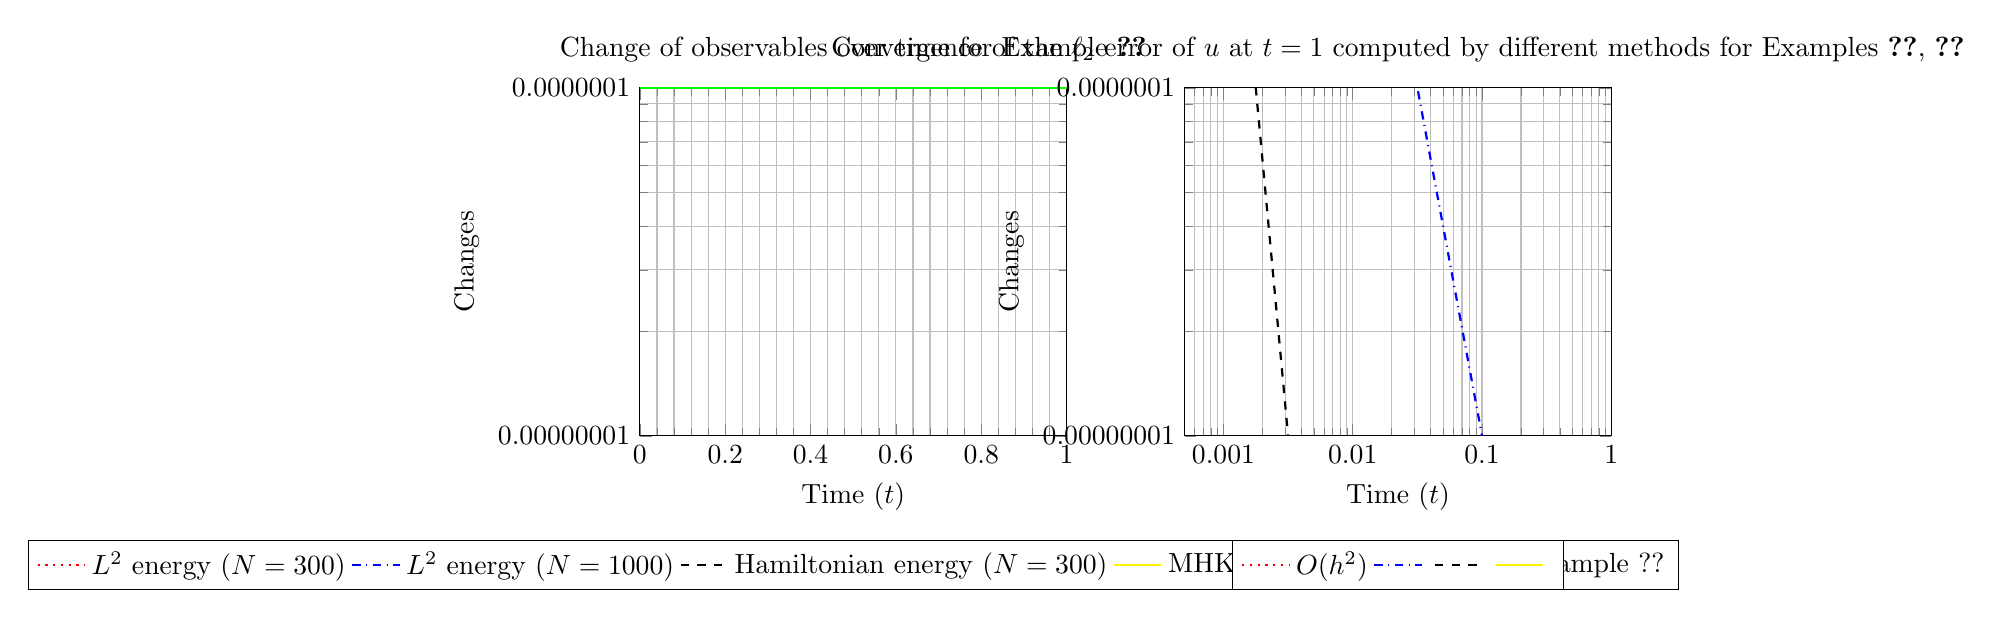
\begin{tikzpicture}
    \begin{groupplot}[
        group style={
            group size=2 by 1,
            horizontal sep=1.5cm
        },
        width=7cm,
        height=6cm,
        grid=both,
        minor tick num=4,
        xmajorgrids=true,
        ymajorgrids=true,
        xmin=0, xmax=1,
        ymin=1e-8, ymax=1e-7,
        xlabel={Time ($t$)},
        ylabel={Changes},
        axis background/.style={fill=white},
        log ticks with fixed point,
        every axis plot post/.append style={mark options={solid}},
        legend style={at={(0.5,-0.3)}, anchor=north,legend columns=-1},
        cycle list name=color list % Use default color cycle
    ]

    % Left plot: Change of observables over time
    \nextgroupplot[
        ymode=log,
        title={Change of observables over time for Example \ref{ex: matrix, nonlinear, time-independent}}
    ]
    \addplot+[dotted, thick] coordinates {
        (0, 1e-7)
        (0.2, 1e-7)
        (0.4, 1e-7)
        (0.6, 1e-7)
        (0.8, 1e-7)
        (1, 1e-7)
    };
    \addlegendentry{$L^2$ energy ($N=300$)}
    
    \addplot+[dashdotted, thick] coordinates {
        (0, 1e-7)
        (0.2, 1e-7)
        (0.4, 1e-7)
        (0.6, 1e-7)
        (0.8, 1e-7)
        (1, 1e-7)
    };
    \addlegendentry{$L^2$ energy ($N=1000$)}
    
    \addplot+[dashed, thick] coordinates {
        (0, 1e-7)
        (0.2, 1e-7)
        (0.4, 1e-7)
        (0.6, 1e-7)
        (0.8, 1e-7)
        (1, 1e-7)
    };
    \addlegendentry{Hamiltonian energy ($N=300$)}
    
    \addplot+[solid, thick] coordinates {
        (0, 1e-7)
        (0.2, 1e-7)
        (0.4, 1e-7)
        (0.6, 1e-7)
        (0.8, 1e-7)
        (1, 1e-7)
    };
    \addlegendentry{MHK Example ??}
    
    \addplot+[solid, thick, green] coordinates {
        (0, 1e-7)
        (0.2, 1e-7)
        (0.4, 1e-7)
        (0.6, 1e-7)
        (0.8, 1e-7)
        (1, 1e-7)
    };
    \addlegendentry{MHK Example ??}
    
    % Right plot: Convergence of $\ell_2$ error
    \nextgroupplot[
        ymode=log,
        xmode=log,
        title={Convergence of the $\ell_2$ error of $u$ at $t=1$ computed by different methods for Examples \ref{ex: matrix, nonlinear, time-dependent}, \ref{ex: matrix, nonlinear, time-independent}}
    ]
    \addplot+[dotted, thick] coordinates {
        (1e-3, 1e-2)
        (1e-2, 1e-3)
        (1e-1, 1e-4)
    };
    \addlegendentry{$O(h^2)$}
    
    \addplot+[dashdotted, thick] coordinates {
        (1e-3, 1e-4)
        (1e-2, 1e-6)
        (1e-1, 1e-8)
    };
    \addlegendentry{}
    
    \addplot+[dashed, thick] coordinates {
        (1e-3, 1e-6)
        (1e-2, 1e-10)
        (1e-1, 1e-14)
    };
    \addlegendentry{}
    
    \addplot+[solid, thick] coordinates {
        (1e-3, 1e-8)
        (1e-2, 1e-16)
        (1e-1, 1e-32)
    };
    \addlegendentry{}
    
    \end{groupplot}
\end{tikzpicture}

\end{document}